\documentclass[10pt, titlepage]{article}
% preámbulo
\usepackage{lmodern}
\usepackage[T3,T1]{fontenc}
\usepackage[document]{ragged2e}
\usepackage[spanish,activeacute]{babel}
\usepackage{mathtools}
\usepackage{hyperref}
\usepackage{xcolor}
\usepackage{geometry}
\usepackage{float}

% Para símbolos fonéticos de la IPA
\usepackage[T1]{tipa}

\geometry{
    a4paper,
    left=25mm,
    right=25mm,
    top=25mm,
    bottom=25mm
}
\usepackage{fancyhdr}

\pagestyle{fancy}
\fancyhf{}
\rhead{Eduardo Arroyo Ramírez \\ i12arrae@uco.es}
\lhead{Software Libre y Compromiso Social \\ Memoria de prácticas}
\lfoot{\rightmark}
\rfoot{Página \thepage}

\def\code#1{\texttt{#1}}

\hypersetup{
    colorlinks=true,
    linkcolor=blue,
    filecolor=magenta,
    urlcolor=cyan,
}

\title{Software Libre y Compromiso Social - Memoria de prácticas}
\author{Eduardo Arroyo Ramírez}

\begin{document}

\graphicspath{ {Practica1/capturas/} }
\graphicspath{ {Practica2/capturas/} }
\graphicspath{ {Practica3/capturas/} }
\graphicspath{ {Practica4/capturas/} }
\graphicspath{ {Practica5/capturas/} }
\graphicspath{ {Practica6/capturas/} }

\makeatletter
\begin{titlepage}
    \begin{center}
        {\scshape\Large Escuela Politécnica Superior \par}
        \vspace{0.5cm}
        {\scshape\large Universidad de Córdoba \par}
        \vspace{4cm}
        {\scshape\Huge Software Libre y Compromiso Social \par}
        \vspace{0.5cm}
        {\itshape\Large Memoria de prácticas \par}
    \end{center}
    \vspace{13cm}
    \begin{flushright}
        \@author\space \\
        i12arrae@uco.es \\
        Curso 2019/2020
    \end{flushright}
\end{titlepage}

\tableofcontents
\listoffigures
\listoftables

% Aquí comienza el cuerpo del documento
\justify
\part{Práctica 1}
\section{Ejercicio 1}
\begin{center}
    \parbox{12cm}{\justify\textit{Elabora una lista de 10 proyectos destacados de software libre y describir los siguientes aspectos de cada uno de esos proyectos:
    \begin{enumerate}
        \item Nombre, página web, autor o autores principales.
        \item Tamaño de la comunidad que lo mantiene. ¿Es mucho o poco activa dicha comunidad?.
        \item ¿Hay alguna empresa privada en torno al proyecto?.
        \item Forma de financiación.
        \item Tipo de licencia de software libre que utiliza el proyecto.
        \item Modelo de desarrollo, lenguaje de programación, sistema operativo y/o plataforma, etc.
        \item Descripción general del proyecto. Escribe 3 o 4 párrafos que describen el proyecto, su funcionalidad y su utilidad.
    \end{enumerate}
    }}
\end{center}
\subsection{Apache}
\begin{enumerate}
    \item Web: \url{https://httpd.apache.org/}. \\ Autores principales: \url{https://httpd.apache.org/contributors/}.
    \item Según la web de apache, la comunidad está formada por voluntarios y hay aproximadamente 7000 personas que han aportado código. Parece una comunidad muy activa ya que según reza la web, tienen más de 200 millones de líneas de código en revisión y más de 3 millones de commits.
    \item Apache Software Foundation (ASF) es una una fundación creada para dar soporte a los proyectos de software bajo la denominación Apache, incluyendo el popular servidor HTTP Apache. La ASF se formó a partir del llamado Grupo Apache y fue registrada en Delaware (Estados Unidos), en junio de 1999. 
    \item La Apache Software Foundation tiene un programa de esponsorización. Entre los principales sponsors se encuentran empresas de primerísimo nivel como Google, Yahoo, Microsoft, Hewlett-Packard, Facebook, AMD, IBM… Cuentan con un apartado de agradecimiento a los sponsors en su página web. Además admiten donativos individuales.También agradecen a la red de mirrors que facilitan la distribución del software de Apache por todo el mundo y cuyo servicio ofrecen a la ASF sin coste alguno.
    \item Apache 2.0. La licencia de software bajo la cual el software de la fundación Apache es distribuido es una parte distintiva de la historia de Apache HTTP Server y de la comunidad de código abierto. La Licencia Apache permite la distribución de derivados de código abierto y cerrado a partir de su código fuente original. 
    \item Utilizan un modelo de gestión de proyectos al que llaman “The Apache Way. Lo explican bastante en profundidad en este video. El lenguaje utilizado es C. Utilizan Subversion para el control de versiones, aunque también tienen repositorios Git. Existen versiones de Apache para Unix, Linux, BSD, Windows, macOS, y otras. 
    \item El servidor HTTP Apache es un servidor web HTTP de código abierto, para plataformas Unix (BSD, GNU/Linux, etc.), Microsoft Windows, Macintosh y otras, que implementa el protocolo HTTP/1.1 y la noción de sitio virtual según la normativa RFC 2616. Cuando comenzó su desarrollo en 1995 se basó inicialmente en código del popular NCSA HTTPd 1.3, pero más tarde fue reescrito por completo. La arquitectura del servidor Apache es muy modular. El servidor consta de una sección core y diversos módulos que aportan mucha de la funcionalidad que podría considerarse básica para un servidor web.
\end{enumerate}
\subsection{Git}
\begin{enumerate}
    \item Web: \url{https://git-scm.com/} Autor: Linus Torvalds, Supervisor: Junio Hamano
    \item Según Wikipedia, la comunidad está formada por alrededor de 280 programadores. La web principal tiene un apartado con instrucciones para la comunidad, que se comunica principalmente mediante listas de correo. A juzgar por las fechas de los mensajes en el archivo y los 58562 commits al proyecto principal en github, la comunidad es realmente activa.
    \item En la página principal se cita una lista de empresas y proyectos que utilizan git. Entre los que destacan Google, Facebook, Microsoft, Twitter, LInkedIn o Netflix.
    \item Según la página principal, Git es miembro de la Software Freedom Conservancy, que según su web es una organización sin ánimo de lucro que promueve, mejora, desarrolla y defiende proyectos software gratuitos, libres y de código abierto (FLOSS). A su vez, esta organización se financia mediante sponsors y donaciones de pequeñas empresas y particulares.
    \item La propia web de git tiene un apartado que explica que Git se licencia bajo GPLv2 “to guarantee your freedom to share and change free software---to make sure the software is free for all its users”. También especifican que el uso del término “Git” y los logos está restringido.
    \item Git está desarrollado en C y Perl principalmente, aunque existen implementaciones escritas en otros lenguajes. Existen versiones de Git para Linux, Windows, BSD, Solaris y macOS.
    \item Git es un software de control de versiones diseñado pensando en la eficiencia y la confiabilidad del mantenimiento de versiones de aplicaciones cuando éstas tienen un gran número de archivos de código fuente. Su propósito es llevar registro de los cambios en archivos de computadora y coordinar el trabajo que varias personas realizan sobre archivos compartidos.
\end{enumerate}


\subsection{LibreOffice}
\begin{enumerate}
    \item Web: \url{https://es.libreoffice.org/}. \\Autores principales: \url{https://es.libreoffice.org/comunidad/desarrolladores/}
    \item La comunidad se divide en varios equipos diferenciados: desarrollo, documentación, infraestructura, diseño, traducción, control de calidad y publicidad. 
    \item The Document Foundation es dirigida e impulsada por sus miembros. Su misión es apoyar y fomentar el desarrollo y el proyecto LibreOffice, así como la su representación.
    \item Reciben donaciones a través de esta página para costear los servidores y la infraestructura.
    \item El proyecto LibreOffice emplea una licencia dual LGPLv3 (o posterior) / MPL para nuevas contribuciones a fin de permitir que la licencia sea actualizada.
    \item En su desarrollo se utilizan los lenguajes C++, Java y Python. Utilizan Git como sistema de control de versiones y el trabajo se administra con Gerrit. Existen versiones de la suite para Windows, macOS y GNU/Linux.
    \item LibreOffice es un paquete de software de oficina. Se creó en 2010 como bifurcación de OpenOffice.org, otro antiguo proyecto de código abierto, que a su vez tenía como base inicial a la suite ofimática StarOffice, desarrollada por StarDivision, adquirida por Sun Microsystems en agosto de 1999. 
\end{enumerate}

\subsection{Gimp}
\begin{enumerate}
    \item The GNU Manipulation Program. Web: \url{s://www.gimp.org/}. Autores principales: Originalmente Spencer Kimball and Peter Mattis. La persona actualmente a cargo es Michael Natterer. Øyvind Kolås es el desarrollador principal de GEGL, el núcleo de GIMP. En esta página se puede encontrar una lista completa de las personas que han contribuido al código de GIMP.
    \item La comunidad se organiza en torno a una wiki y un canal de IRC. Además existen multitud de foros de usuarios. La comunidad de desarrollo es bastante activa a juzgar por las fechas de las entradas en la web de seguimiento en Gitlab. En la página sobre el desarrollo hay un gráfico que muestra una actividad constante en los últimos 5 años de commits, y además reza que hay un total de 72 contribuyentes activos.
    \item GIMP forma parte del proyecto GNU. La fundación GNOME ayuda a GIMP canalizando las donaciones al proyecto GIMP a través de su organización..
    \item El proyecto se financia mediante donaciones a través de plataformas de pago como Paypal. Además, Øyvind Kolås y Jehan Pagès tienen sendas páginas de mecenazgo donde reciben donaciones por su trabajo en GEGL y para el desarrollo de funcionalidades de animación en GIMP respectivamente.
    \item GPLv3+ y LGPL
    \item Está escrito en C y utiliza GTK. Utilizan Git como sistema de control de versiones, alojado por GNOME Foundation. Está disponible para Unix, GNU/Linux, FreeBSD, Solaris, Windows y macOS entre otros. El desarrollo se gestiona desde una wiki y se utiliza un canal de IRC (\url{irc://irc.gimp.org/#gimp}) para la comunicación directa entre desarrolladores.
    \item GIMP (siglas en inglés de GNU Image Manipulation Program) es un programa de edición de imágenes digitales en forma de mapa de bits, tanto dibujos como fotografías. GIMP tiene herramientas que se utilizan para el retoque y edición de imágenes, dibujo de formas libres, cambiar el tamaño, recortar, hacer fotomontajes, convertir a diferentes formatos de imagen, y otras tareas más especializadas. Se pueden también crear imágenes animadas en formato GIF e imágenes animadas en formato MPEG usando un plugin de animación.
\end{enumerate}


\subsection{Symphony}
\begin{enumerate}
    \item Web: \url{https://symfony.com}. Líder actual del proyecto: Fabien Potencier
    \item Según la web del proyecto, hay más de 600.000 desarrolladores implicados. Parece una comunidad muy activa.
    \item Symfony es patrocinado por SensioLabs, una compañía francesa que provee consultoría, servicios, formación sobre tecnologías open source.
    \item Symfony está financiado por SensioLabs
    \item Utiliza licencia MIT
    \item Está desarrollado en PHP y se puede utilizar en plataformas Unix, GNU/Linux, macOS y Windows.
    \item Symfony es un framework diseñado para desarrollar aplicaciones web basado en el patrón Modelo Vista Controlador. Para empezar, separa la lógica de negocio, la lógica de servidor y la presentación de la aplicación web. Proporciona varias herramientas y clases encaminadas a reducir el tiempo de desarrollo de una aplicación web compleja. Además, automatiza las tareas más comunes, permitiendo al desarrollador dedicarse por completo a los aspectos específicos de cada aplicación.
\end{enumerate}


\subsection{Node.js}
\begin{enumerate}
    \item Web: nodejs.org. Autor:  Ryan Dahl
    \item La comunidad es muy activa en los grupos de google como nodejs, nodejs-dev y también su canal de IRC \#node.js en freenode. Se reúnen en la NodeConf.
    \item OpenJS Foundation / Joyent
    \item No he encontrado información acerca del modelo de financiación del proyecto.
    \item Licencia MIT.
    \item El cuerpo de operaciones de base de Node.js está escrito en JavaScript con métodos de soporte escritos en C++. Utiliza el motor javascript V8 originalmente creado para Google Chrome, que está escrito en C++. NodeJS está disponible para sistemas Unix, GNU/Linux, macOS, Windows...
    \item Node.js es un entorno en tiempo de ejecución multiplataforma, de código abierto, para la capa del servidor (pero no limitándose a ello) basado en el lenguaje de programación ECMAScript, asíncrono, con E/S de datos en una arquitectura orientada a eventos y basado en el motor V8 de Google. Fue creado con el enfoque de ser útil en la creación de programas de red altamente escalables, como por ejemplo, servidores web.
\end{enumerate}


\subsection{Ubuntu}
\begin{enumerate}
    \item Web: \url{https://ubuntu.com/}. Autor
    \item La comunidad se coordina desde \url{https://discourse.ubuntu.com/}. Ésta participa en el desarrollo, arreglo de bugs, traducción, documentación, etc. No he encontrado datos sobre el tamaño de la comunidad.
    \item Canonical
    \item Ubuntu se financia principalmente a través de la actividad de Canonical.
    \item GPL y otras licencias libres
    \item Según la guía de instalación, Ubuntu soporta las seis arquitecturas principales (x86, x64, ARM, ARM64, IBM POWER e IBM z, y muchas de sus variantes.\\Además de la arquitectura IBM/Motorola PowerPC, que tiene un port no oficial.
    \item Ubuntu es un sistema operativo de código abierto y libre para computadores. Es una distribución de Linux basada en Debian. Actualmente corre en computadores de escritorio y servidores. Está orientado al usuario promedio, con un fuerte enfoque en la facilidad de uso y en mejorar la experiencia del usuario. Está compuesto de múltiple software normalmente distribuido bajo una licencia libre o de código abierto.
    
    Estadísitcas web sugieren que la cuota de mercado de Ubuntu dentro de las distribuciones Linux es, aproximadamente, del 52\%, y con una tendencia a aumentar como servidor web. Canonical, además de mantener Ubuntu, provee una versión orientada a servidores, Ubuntu Server, una versión para empresas, Ubuntu Business Desktop Remix, una para televisores, Ubuntu TV, otra versión para tabletas Ubuntu Tablet, también Ubuntu Phone y una para usar el escritorio desde teléfonos inteligentes, Ubuntu for Android.
\end{enumerate}


\subsection{Gnome}
\begin{enumerate}
    \item Web: \url{https://www.gnome.org/} Autores:  Miguel de Icaza y Federico Mena 
    \item La comunidad se comunica a través de IRC y listas de correo. No he encontrado un dato del tamaño de la comunidad, pero a juzgar por la lista de cambios recientes y la frecuencia de las actualizaciones, la comunidad de desarrolladores es muy activa.
    \item GNOME Foundation (parte de GNU Project)
    \item GNOME Se financia a través de sus patrocinadores como Canonical, Debian, Google, RedHat, EndlessOS, SUSE y otros. También recibe donaciones particulares.
    \item licencia
    \item GNOME está escrito principalmente en C y C++. GNOME está disponible en las principales distribuciones GNU/Linux, incluyendo Fedora, Debian, Ubuntu, Red Hat Linux, CentOS, Oracle Linux, Arch Linux y Gentoo.
    \item GNOME provee un gestor de ventanas «intuitivo y atractivo» y una plataforma de desarrollo para crear aplicaciones que se integran con el escritorio. El Proyecto pone énfasis en la simplicidad, facilidad de uso y eficiencia. Tiene como objetivo la libertad para crear un entorno de escritorio que siempre tendrá el código fuente disponible para reutilizarse bajo una licencia de software libre.
    
    Desde GNOME 2, el enfoque fue puesto en la productividad. Con este fin, se crearon las Pautas de Interfaz Humana de GNOME (Human Interface Guidelines, HIG). Todos los programas de GNOME comparten un estilo coherente de interfaz gráfica de usuario (GUI), pero no están limitados a los mismos widgets de GUI. Por el contrario, el diseño de la GUI de GNOME está guiado por conceptos que se describen en GNOME HIG, que a su vez depende de la ergonomía cognitiva. Después de HIG, los desarrolladores pueden crear programas de GUI de alta calidad, consistentes y utilizables, ya que abordan todo, desde el diseño de la GUI hasta el diseño recomendado de widgets basado en píxeles.
\end{enumerate}


\subsection{GCC}
\begin{enumerate}
    \item Web: \url{https://www.gnu.org/software/gcc/}. Autor: Proyecto  GNU
    \item GCC mantiene una larguísima lista de colaboradores en su web \\\url{https://gcc.gnu.org/onlinedocs/gcc/Contributors.html}
    \item Free Software Foundation
    \item La FSF recibe financiación de sus ``patrons'' y de donaciones particulares.
    \item GPLv3
    \item Gcc está escrito en C
    \item El GNU Compiler Collection (colección de compiladores GNU) es un conjunto de compiladores creados por el proyecto GNU. GCC es software libre y lo distribuye la Free Software Foundation (FSF) bajo la licencia general pública GPL. Estos compiladores se consideran estándar para los sistemas operativos derivados de UNIX, de código abierto y también de propietarios, como Mac OS X. GCC requiere el conjunto de aplicaciones conocido como binutils para realizar tareas como identificar archivos objeto u obtener su tamaño para copiarlos, traducirlos o crear listas, enlazarlos, o quitarles símbolos innecesarios. Originalmente GCC significaba GNU C Compiler (compilador GNU de C), porque solo compilaba el lenguaje C. Posteriormente se extendió para compilar C++, Fortran, Ada y otros.
\end{enumerate}


\subsection{React}
\begin{enumerate}
    \item Web \url{https://reactjs.org/}, Autor: Jordan Walke
    \item La comunidad es grande y activa
    \item Facebook Inc.
    \item Es financiado por Facebook.
    \item Actualmente MIT, aunque empezó con ApacheV2 y luego paso a BSD de 3 cláusulas.
    \item Desarrollado en Javascript. React es una biblioteca javascript para web, por lo que es soportado por cualquiera de los navegadores modernos.
    \item React (también llamada React.js o ReactJS) es una biblioteca Javascript de código abierto diseñada para crear interfaces de usuario con el objetivo de facilitar el desarrollo de aplicaciones en una sola página. Es mantenido por Facebook y la comunidad de software libre, han participado en el proyecto más de mil desarrolladores diferentes. React intenta ayudar a los desarrolladores a construir aplicaciones que usan datos que cambian todo el tiempo. Su objetivo es ser sencillo, declarativo y fácil de combinar.\\React sólo maneja la interfaz de usuario en una aplicación; React es la Vista en un contexto en el que se use el patrón MVC (Modelo-Vista-Controlador) o MVVM (Modelo-vista-modelo de vista). También puede ser utilizado con las extensiones de React-based que se encargan de las partes no-UI (que no forman parte de la interfaz de usuario) de una aplicación web.
\end{enumerate}

\clearpage
\section{Ejercicio 2}

\begin{center}
    \parbox{12cm}{\justify\textit{Familiarízate con las comunidades de proyectos emblemáticos y también personajes del software libre como son:
\begin{enumerate}
    \item Free Software Movement. Breve descripción y describe alguna de sus iniciativas.
    \item Open Source Initiative. Describe alguna de sus iniciativas.
    \item Diferencias entre Free Software Foundation y GNU Project
    \item Describe brevemente algunos de los principales proyectos que se traen entre manos en proyecto GNU
    \item Linux distros: Debian, Ubuntu, Mint
    \item Analiza y describe brevemente las figuras de Richard Stallman (GNU), Linus Torvalds (Linux), Eric S. Raymond (“La Catedral y el Bazar”). Añade dos figuras más (en total serían 5) que han aportado al mundo del Software libre y escribe una breve descripción de ellas. 
\end{enumerate}
    }}
\end{center}

\subsection{Free Software Movement}
El movimiento del software libre es un movimiento social con el objetivo de obtener y garantizar las libertades que permiten a los usuarios de software ejecutarlo, estudiarlo, cambiarlo y redistribuir copias del mismo con o sin cambios.

Sobre la base de las tradiciones y filosofías de la cultura hacker y el mundo académico de los años 1970s, Richard Stallman fundó formalmente el movimiento en 1983, con el lanzamiento del Proyecto GNU. Stallman estableció la Fundación del Software Libre en 1985 para apoyar el movimiento. La meta del movimiento fue dar libertad a los usuarios, reemplazando el software con términos de licencia restrictivos, como el software privativo, por software libre.

\subsection{Open Source Initiative}
La Open Source Initiative es una organización (public benefit corporation) californiana fundada en el año 1998 por Bruce Perens y Eric S. Raymond, que promueve el uso de software de código abierto.

\subsection{Diferencias entre la FSF y GNU Project}
La Free Software Foundation es una organización sin ánimo de lucro con la misión de promover la libertad de los usuarios de computadoras. Defienden los derechos de todos los usuarios de software y centra su trabajo en asuntos legales, organizativos y promocionales en beneficio de la comunidad de usuarios de software libre. Por su parte, el Proyecto GNU es un proyecto colaborativo con el objetivo de crear un sistema operativo completamente libre, incluyendo sus herramientas de aplicación.

El objetivo inicial de la Free Software Foundation era recaudar fondos para ayudar a programar GNU.

\subsection{Principales proyectos GNU}
El Proyecto GNU consta de una serie de pequeños subproyectos mantenidos por voluntarios, empresas o combinaciones de ambos. Estos subproyectos también se denominan «Proyectos de GNU» o «Paquetes GNU». Algunos de los más conocidos son:

\subsubsection{GCC}
El GNU Compiler Collection (colección de compiladores GNU) es un conjunto de compiladores creados por el proyecto GNU. GCC es software libre y lo distribuye la Free Software Foundation (FSF) bajo la licencia general pública GPL.
Estos compiladores se consideran estándar para los sistemas operativos derivados de UNIX, de código abierto y también de propietarios, como Mac OS X. GCC requiere el conjunto de aplicaciones conocido como binutils para realizar tareas como identificar archivos objeto u obtener su tamaño para copiarlos, traducirlos o crear listas, enlazarlos, o quitarles símbolos innecesarios.
Originalmente GCC significaba GNU C Compiler (compilador GNU de C), porque solo compilaba el lenguaje C. Posteriormente se extendió para compilar C++, Fortran, Ada y otros.

GCC es parte del proyecto GNU, y tiene como objetivo mejorar el compilador usado en todos los sistemas GNU, incluyendo la variante GNU/Linux. El desarrollo de GCC usa un entorno de desarrollo abierto y soporta muchas plataformas con el fin de fomentar el uso de un compilador-optimizador de clase global, que pueda atraer muchos equipos de desarrollo, y asegure que GCC y los sistemas GNU funcionen en diferentes arquitecturas y diferentes entornos, y más aún, para extender y mejorar las características de GCC.

\subsubsection{GNOME}
GNOME es un entorno de escritorio e infraestructura de desarrollo para sistemas operativos Unix,  GNU/Linux y derivados Unix como BSD o Solaris; compuesto enteramente de software libre.

El proyecto fue iniciado por los programadores mexicanos Miguel de Icaza y Federico Mena en agosto de 1997 y forma parte oficial del proyecto GNU. Nació como una alternativa a KDE bajo el nombre de GNU Network Object Model Environment (Entorno de Modelo de Objeto de Red GNU). Actualmente, incluyendo al español, se encuentra disponible en 166 idiomas.

GNOME está disponible en las principales distribuciones GNU/Linux, incluyendo Fedora, Debian, Ubuntu, Red Hat Linux, CentOS, Oracle Linux, Arch Linux y Gentoo.

\subsubsection{Bash}
GNU Bash o simplemente Bash (Bourne-again shell) es un lenguaje de comandos y shell de Unix escrito por Brian Fox para el Proyecto GNU como un reemplazo de software libre para el shell Bourne. Lanzado por primera vez en 1989, se ha utilizado ampliamente como el shell de inicio de sesión predeterminado para la mayoría de las distribuciones de Linux y MacOS Mojave de Apple y versiones anteriores. Una versión también está disponible para Windows 10 y Android. También es el shell de usuario predeterminado en Solaris 11.

Bash es un procesador de comandos que generalmente se ejecuta en una ventana de texto donde el usuario escribe comandos que causan acciones. Bash también puede leer y ejecutar comandos desde un archivo, llamado script de shell. Al igual que todos los shells de Unix, es compatible con el agrupamiento de nombres de archivo (coincidencia de comodines), tuberías, here documents, sustitución de comandos, variables y estructuras de control para pruebas de condición e iteración. Las palabras reservadas, la sintaxis, las variables de ámbito dinámico y otras características básicas del lenguaje se copian de sh. Otras características, por ejemplo, el historial, se copian de csh y ksh. Bash es un shell compatible con POSIX, pero con varias extensiones.

\subsubsection{GIMP}
GIMP (siglas en inglés de GNU Image Manipulation Program) es un programa de edición de imágenes digitales en forma de mapa de bits, tanto dibujos como fotografías. Es un programa libre y gratuito. Forma parte del proyecto GNU y está disponible bajo la Licencia pública general de GNU y GNU Lesser General Public License.

Es el programa de manipulación de gráficos disponible en más sistemas operativos (Unix, GNU/Linux, FreeBSD, Solaris, Microsoft Windows y macOS, entre otros).

GIMP tiene herramientas que se utilizan para el retoque y edición de imágenes, dibujo de formas libres, cambiar el tamaño, recortar, hacer fotomontajes, convertir a diferentes formatos de imagen, y otras tareas más especializadas. Se pueden también crear imágenes animadas en formato GIF e imágenes animadas en formato MPEG usando un plugin de animación.

Los desarrolladores y encargados de mantener GIMP se esfuerzan en mantener y desarrollar una aplicación gráfica de software libre, de alta calidad para la edición y creación de imágenes originales, de fotografías, de íconos, de elementos gráficos tanto de páginas web como de elementos artísticos de interfaz de usuario.

\subsection{Distribuciones Linux}

\subsubsection{Debian}
Debian o Proyecto Debian, (en inglés, Debian Project) es una comunidad conformada por desarrolladores y usuarios, que mantiene un sistema operativo GNU basado en software libre. El sistema se encuentra precompilado, empaquetado y en formato deb para múltiples arquitecturas de computador y para varios núcleos.

El proyecto Debian fue anunciado inicialmente 1993 por Ian Murdock. El nombre Debian proviene de la combinación del nombre de su entonces novia (y posteriormente ex-esposa) Deborah y el suyo, por lo tanto, Deb(orah) e Ian. Debian 0.01 fue lanzado el 15 de septiembre de 1993, y la primera versión estable fue hecha en 1996.

Nació como una apuesta por separar en sus versiones el software libre del software no libre. El modelo de desarrollo del proyecto es ajeno a motivos empresariales o comerciales, siendo llevado adelante por los propios usuarios, aunque cuenta con el apoyo de varias empresas en forma de infraestructuras. Debian no vende directamente su software, lo pone a disposición de cualquiera en Internet, aunque sí permite a personas o empresas distribuirlo comercialmente mientras se respete su licencia.

La comunidad de desarrolladores del proyecto cuenta con la representación de Software in the Public Interest (del inglés, "software de interés público"), una organización sin ánimo de lucro que da cobertura legal a varios proyectos de software libre, con el objetivo inicial de dar cobertura legal al proyecto Debian, tras el fin del patrocinio de la FSF (Free Software Foundation).

La primera adaptación del sistema Debian, siendo también la más desarrollada, es Debian GNU/Linux, basada en el núcleo Linux, y como siempre utilizando herramientas de GNU. Existen también otras adaptaciones con diversos núcleos: Hurd (Debian GNU/Hurd); NetBSD (Debian GNU/NetBSD) y FreeBSD (Debian GNU/kFreeBSD).

\subsubsection{Ubuntu}
Ubuntu es un sistema operativo de código abierto y libre para computadores. Es una distribución de Linux basada en Debian. Actualmente corre en computadores de escritorio y servidores. Está orientado al usuario promedio, con un fuerte enfoque en la facilidad de uso y en mejorar la experiencia del usuario. Está compuesto de múltiple software normalmente distribuido bajo una licencia libre o de código abierto. Estadísticas web sugieren que la cuota de mercado de Ubuntu dentro de las distribuciones Linux es, aproximadamente, del 52 \%, y con una tendencia a aumentar como servidor web.

Su patrocinador, Canonical, es una compañía británica propiedad del empresario sudafricano Mark Shuttleworth. Ofrece el sistema de manera gratuita, y se financia por medio de servicios vinculados al sistema operativo y vendiendo soporte técnico. Además, al mantenerlo libre y gratuito, la empresa es capaz de aprovechar los desarrolladores de la comunidad para mejorar los componentes de su sistema operativo. Extraoficialmente, la comunidad de desarrolladores proporciona soporte para otras derivaciones de Ubuntu, con otros entornos gráficos, como Kubuntu, Xubuntu, Ubuntu MATE, Edubuntu, Ubuntu Studio, Mythbuntu, Ubuntu GNOME y Lubuntu.Canonical, además de mantener Ubuntu, provee una versión orientada a servidores, Ubuntu Server, una versión para empresas, Ubuntu Business Desktop Remix, una para televisores, Ubuntu TV, otra versión para tabletas Ubuntu Tablet, también Ubuntu Phone y una para usar el escritorio desde teléfonos inteligentes, Ubuntu for Android.

Cada seis meses se publica una nueva versión de Ubuntu. Esta recibe soporte por parte de Canonical durante nueve meses por medio de actualizaciones de seguridad, parches para bugs críticos y actualizaciones menores de programas. Las versiones LTS (Long Term Support), que se liberan cada dos años, reciben soporte durante cinco años en los sistemas de escritorio y de servidor.

\subsubsection{Mint}
Linux Mint es una distribución de GNU/Linux comunitaria de origen franco-irlandesa basada en Debian y Ubuntu que tiene por objeto proveer "un sistema operativo moderno, elegante y cómodo que sea tan potente como fácil de usar". Linux Mint soporta multimedia al incluir software propietario y empaquetado con una variedad de aplicaciones gratuitas y de código abierto.

El proyecto fue concebido por Clément Lefèbvre y está siendo activamente desarrollado por el Equipo de Linux Team y la comunidad.

\subsection{Figuras del Software Libre}

\subsubsection{Richard Stallman}
Richard Matthew Stallman (Manhattan, Nueva York, 16 de marzo de 1953), con frecuencia abreviado como «rms», es un programador estadounidense y fundador del movimiento del software libre.

Entre sus logros destacados como programador se incluye la realización del editor de texto GNU Emacs, el compilador GCC, el depurador GDB, y el lenguaje de construcción GNU Make; todos bajo la rúbrica del Proyecto GNU. Sin embargo, es principalmente conocido por el establecimiento de un marco de referencia moral, político y legal para el software libre: un modelo de desarrollo y distribución alternativo al software privativo. Es también inventor del concepto de copyleft (aunque no del término): un método para licenciar obras contempladas por el derecho de autor, de tal forma que su uso y modificación (así como de sus derivados) permanezcan siempre permitidos.

\subsubsection{Linus Torvalds}
Linus Benedict Torvalds (Helsinki, Finlandia, 28 de diciembre de 1969) es un ingeniero de software finlandés-estadounidense, conocido por iniciar y mantener el desarrollo del kernel (en español, núcleo) Linux, basándose en el sistema operativo libre Minix creado por Andrew S. Tanenbaum y en algunas herramientas, varias utilidades y los compiladores desarrollados por el proyecto GNU. Actualmente es responsable de la coordinación del proyecto.

\subsubsection{Eric S. Raymond}
Eric Steven Raymond (nacido el 4 de diciembre de 1957), también conocido como ESR, es el autor de La catedral y el bazar, (``The Cathedral \& the Bazaar'', en inglés) y el responsable actual del Jargon File (también conocido como The New Hacker's Dictionary). Si bien con el Jargon File obtuvo fama como historiador de la cultura hacker, se convirtió después de 1997 en una figura líder en el Movimiento del Open Source y el Código abierto. Hoy día es uno de sus personajes más famosos y controvertidos.

Raymond es un neopagano, un confeso anarcocapitalista, y un defensor del derecho a poseer y utilizar armas de fuego. Tiene un gran interés en la ciencia ficción. Es músico amateur y cinturón negro de taekwondo.

\subsubsection{Guido van Rossum}
Guido van Rossum es un informático, conocido por ser el autor del lenguaje de programación Python. Nació y creció en los Países Bajos.

En el ambiente de los desarrolladores del lenguaje Python también se le conoce por el título BDFL (Benevolent Dictator for Life), teniendo asignada la tarea de fijar las directrices sobre la evolución de Python, así como la de tomar decisiones finales sobre el lenguaje que todos los desarrolladores acatan. Van Rossum tiene fama de ser bastante conservador, realizando pocos cambios al lenguaje entre versiones sucesivas, intentando mantener siempre la compatibilidad con versiones anteriores. El 12 de julio de 2018, con un mensaje enviado a la lista de python-committers, anunció su retiro de los procesos de decisión.

En el año 2001 recibió el FSF Award for the Advancement of Free Software como reconocimiento por su trabajo. En diciembre de 2005 fue contratado como desarrollador por la empresa estadounidense Google. Después de siete años en Google, a principios de diciembre de 2012, anuncia su retirada de la empresa norteamericana para incorporarse en enero de 2013 a la plantilla de la compañía Dropbox.

\subsubsection{Ian Murdock}
Ian Ashley Murdock (Konstanz, Alemania, 28 de abril de 1973-28 de diciembre de 2015) fue un informático estadounidense y fundador del proyecto de software libre Debian.

En 1993 escribió el Manifiesto Debian mientras estudiaba en la Purdue University, donde en 1996 obtuvo su licenciatura. Fue fundador, también, de la empresa Progeny Linux Systems. Fue CTO de la Linux Foundation y líder del Proyecto Indiana cuando trabajaba para Sun Microsystems.
% \part{Práctica 2}
% \part{Práctica 3}
Siguiendo las instrucciones del enunciado, la práctica 3 se ha realizado en un documento de LibreOffice Writer y se puede descargar del \href{http://www.google.es}{repositorio de github}.
% \part{Práctica 4}

\section{Ejercicio 1}
\begin{center}
    \parbox{12cm}{\justify\textit{Uso extendido de GNU/Linux en escritorio y en la industria. Últimos avances.
    Lectura recomendada:
    \begin{itemize}
        \item \href{https://hipertextual.com/2018/12/snaps-instalar-software-linux}{Snaps: ¿El método más simple para instalar apps en Linux?}
    \end{itemize}
    Cuestiones:
    \begin{enumerate}
    \item Porcentaje de uso de los principales SO de escritorio.
    \item ¿Cómo crees que podría mejorarse el uso de GNU/Linux en escritorios?
    \item ¿Qué es snap y snapcraft.io? ¿para qué sirve y qué diferencias aporta al sistema tradicional de instalación de paquetes de GNU/Linux?
    \item Buscar cómo se instala snap en mi distribución en la documentación de snap.
    \item Instalar y probar snap
    \item ¿Crees que mejora en el sentido de facilitar el uso de GNU/Linux?
    \end{enumerate}}}
\end{center}

\subsection{Pregunta 1}
Estos gráficos muestran los datos de abril de 2020 sobre el porcentaje de uso de los principales SO de escritorio en todo el mundo \cite{statcounter:os_share_worldwide} y en España \cite{statcounter:os_share_spain}.
\begin{figure}[H]
    \centering
    \begin{tikzpicture}    
        \pie [cloud, scale font, radius=2, text=legend]
        {76.5/Windows, 18.99/OS X, 1.61/Linux, 1.12/Chrome OS, 1.75/Otros}
    \end{tikzpicture}
    \caption{Uso de los principales SO de escritorio en abril de 2020 en el mundo.}\label{fig:uso-so-mundial}
\end{figure}
\begin{figure}[H]
    \centering
    \begin{tikzpicture}    
        \pie [cloud, scale font, radius=2, text=legend]
        {76.1/Windows, 20.62/OS X, 1.71/Linux, 0.46/Chrome OS, 1.11/Otros}
    \end{tikzpicture}
    \caption{Uso de los principales SO de escritorio en abril de 2020 en España.}\label{fig:uso-so-españa}
\end{figure}

\subsection{Pregunta 2}
Creo que el porcentaje de uso de GNU/Linux aumentaría significativamente a largo plazo si las administraciones lo adoptasen ampliamente, sobre todo en el ámbito de la educación. Por otra parte, la mayoría de los ordenadores que se venden incluyen una licencia de Windows como si no hubiera opción. Si se acabase con esta práctica y en su lugar se permitiese al comprador elegir, los usuarios percibirían mejor el valor y el precio del producto que están comprando y, sin duda, muchos elegirían GNU/Linux aunque sólo fuera por el precio.

En mi opinión, la dificultad de uso no es un factor que frene la adopción de GNU/Linux para el usuario medio de hoy. Si algo detiene al usuario a la hora de decidir utilizar un sistema operativo diferente es hábito, el aferrarse a lo que conoce y rechazar el cambio.

\subsection{Pregunta 3}
<<Snap>> es un sistema de gestión de paquetes paquete de aplicación para escritorio, nube o IoT, creado y diseñado por Canonical. \href{http://snapcraft.io}{snapcraft.io} es la herramienta que utilizan los desarrolladores para empaquetar sus programas en formato snap.
La principal ventaja de snap frente a otros sistemas de gestión de paquetes es ser independiente de la distribución en la que se instala. Los propios snaps no dependen de ninguna tienda de aplicaciones y se pueden obtener de cualquier forma. El inconveniente de Snap es el mayor tamaño de sus paquetes, ya que cada uno viene con sus dependencias incluidas.

\subsection{Pregunta 4}
Según las instrucciones para la \href{https://snapcraft.io/docs/installing-snap-on-ubuntu}{instalación de snap en Ubuntu}\footnote{\label{nota1}\url{https://snapcraft.io/docs/installing-snap-on-ubuntu}}, snap se instala por defecto en Ubuntu 20.04, que es la distribución que tengo actualmente instalada.

\subsection{Pregunta 5}
Como snap se instaló automáticamente con mi Ubuntu, paso a comprobar la instalación siguiendo las instrucciones que dan en \href{https://snapcraft.io/docs/installing-snap-on-ubuntu}{snapcraft.io}\footnotemark[1]. En la figura \ref{fig:ubuntu-snap} se puede ver la ejecución del comando snap sin parámetros, la instalación del paquete \code{hello-world} y la ejecución posterior del programa instalado.

\begin{figure}[H]
    \centering
    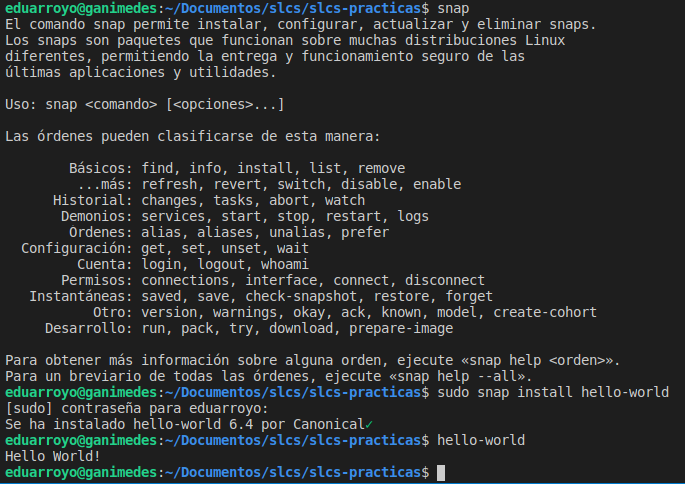
\includegraphics[scale=0.5]{comprobacion-ubuntu-snap}
    \caption{Comprobación de funcionamiento de snap}
    \label{fig:ubuntu-snap}
\end{figure}

\subsection{Pregunta 6}
Al menos en Ubuntu, la tienda de aplicaciones que conocía, junto con \code{apt},  hacían bastante fácil la instalación de aplicaciones en GNU/Linux. Sin duda, el carácter multiplataforma de snap contribuye a una mayor homogeneización del software entre las distintas distribuciones, pero sobre todo facilita el trabajo a los desarrolladores, que sólo tienen que empaquetar sus aplicaciones en un sistema.

\section{Ejercicio 2}
\begin{center}
    \parbox{12cm}{\justify\textit{Free software and GNU/Linux publications:
    \begin{itemize}
    \item LJ. Linux Journal. \url{https://www.linuxjournal.com/}
    \item LM. Linux Magazine. \url{http://www.linux-magazine.com/}
    \item Linux Weekly News. \url{https://lwn.net/}
    \item \url{http://linux.com}
    \item nixCraft. \url{https://www.cyberciti.biz/}
    \item \href{https://slashdot.org}{slashdot} y barrapunto
    \item OMG! Ubuntu!. We follow the Ubuntu and GNOME development. \url{https://www.omgubuntu.co.uk/}
    \item Sección “Linux” en: \url{http://hipertextual.com}
    \item \url{https://ayudalinux.com/}
    \item \url{https://lamiradadelreplicante.com/}
    \end{itemize}
    Cuestiones:
    \begin{enumerate}
    \item Ordena tus preferencias de 1 a 5.
    \item ¿Has encontrado contenido GNU/Linux o de free software en otras publicaciones?¿Cuáles?
    \end{enumerate}
    }}
\end{center}

\subsection{Pregunta 1}
Aunque para valorar las distintas publicaciones haría falta un seguimiento más detenido de cada web, diría que las cinco que más me han gustado son estas:
\begin{enumerate}
    \item OMG! Ubuntu! Tiene un aire desenfadado y artículos no tan técnicos, pero muy interesantes, con novedades y proyectos curiosos.
    \item ayudalinux.com está orientado a quienes se inician con Linux, con muchos tutoriales y artículos para solucionar problemas comunes.
    \item Linux Magazine tiene contenido técnico muy detallado y artículos clasificados por áreas como administración, desarrollo, hardware, servidor, programación..., el problema es que muchos de sus artículos son de pago.
    \item slashdot es una web donde los usuarios envían noticias de temas diversos y las comentan. Tienen un apartado específico con temas de FOSS.
    \item linux.com Es una web de recopilación de noticias clasificadas por temas como Open Source, Seguridad, Administración de sisteams, IoT, Hardware, Linux...
\end{enumerate}

\subsection{Pregunta 2}

\begin{itemize}
    \item \href{https://www.linuxtoday.com/}{Linux Today}
    \item \href{https://www.tecmint.com/}{TecMint}
    \item \href{https://linux.softpedia.com}{Softpedia: Linux}
    \item \href{https://linuxinsider.com/}{Linux Insider}
    \item \href{https://www.cyberciti.biz/}{nixCraft}
\end{itemize}


\section{Ejercicio 3}
\begin{center}
    \parbox{12cm}{\justify\textit{GNU/Linux en redes sociales:
    \begin{itemize}
    \item \href{https://twitter.com/Linux}{@Linux} 269mil
    \item \href{https://twitter.com/usemoslinux}{@usemoslinux} 24mil
    \item \href{https://twitter.com/MuyLinux}{@MuyLinux} 23mil
    \item \href{https://twitter.com/linuxhispano}{@linuxhispano} 7mil
    \item \href{https://twitter.com/andalinux}{@andalinux} 3mil
    \item \href{https://twitter.com/AulaSL}{@AulaSL} 634
    \end{itemize}
    Best Linux hashtags, o hashtags relacionadas con Linux que más se usan en RRSS:
    \href{https://twitter.com/hashtag/linux}{\#linux}
    \href{https://twitter.com/hashtag/programming}{\#programming}
    \href{https://twitter.com/hashtag/python}{\#python}
    \href{https://twitter.com/hashtag/coding}{\#coding}
    \href{https://twitter.com/hashtag/hacking}{\#hacking}
    \href{https://twitter.com/hashtag/technology}{\#technology}
    \href{https://twitter.com/hashtag/programmer}{\#programmer}
    \href{https://twitter.com/hashtag/technology}{\#technology}
    \href{https://twitter.com/hashtag/java}{\#java}
    \href{https://twitter.com/hashtag/hacker}{\#hacker}
    \href{https://twitter.com/hashtag/computerscience}{\#computerscience}
    \href{https://twitter.com/hashtag/code}{\#code}
    \href{https://twitter.com/hashtag/coder}{\#coder}
    \href{https://twitter.com/hashtag/javascript}{\#javascript}
    \href{https://twitter.com/hashtag/html}{\#html}
    \href{https://twitter.com/hashtag/developer}{\#developer}
    \href{https://twitter.com/hashtag/cybersecurity }{\#cybersecurity }
    \href{https://twitter.com/hashtag/webdeveloper}{\#webdeveloper}
    \href{https://twitter.com/hashtag/css}{\#css}
    \href{https://twitter.com/hashtag/computer}{\#computer}
    \href{https://twitter.com/hashtag/kalilinux}{\#kalilinux}
    \href{https://twitter.com/hashtag/software}{\#software}
    \href{https://twitter.com/hashtag/php}{\#php}
    \href{https://twitter.com/hashtag/webdevelopment}{\#webdevelopment}
    \href{https://twitter.com/hashtag/webdesign}{\#webdesign}
    \href{https://twitter.com/hashtag/programmers}{\#programmers}
    \href{https://twitter.com/hashtag/geek}{\#geek}
    \href{https://twitter.com/hashtag/softwaredeveloper}{\#softwaredeveloper}
    \href{https://twitter.com/hashtag/windows}{\#windows}
    \href{https://twitter.com/hashtag/bhfyp}{\#bhfyp}
    \\ Cuestiones:
    \begin{enumerate}
    \item Anota las cuentas de Twitter que más te gusten de las anteriores o de otras que tú consultes en orden preferente de 1 a 5.
    \item ¿Has encontrado contenido GNU/Linux o de free software en otras RRSS? ¿Cuáles?
    \end{enumerate}
    Lectura recomendada en el portal Linux Journal sobre su 25 aniversario:
    \begin{itemize}
        \item \href{https://www.linuxjournal.com/content/25-years-later-interview-linus-torvalds}{25 Years Later: Interview with Linus Torvalds}
    \end{itemize}
    }}
\end{center}

\subsection{Pregunta 1}

\begin{enumerate}
    \item @linuxhispano comparte los artículos de su web \url{http://linuxhispano.net} y también su tira cómica.
    \item @andalinux es muy activo en twitter y comparte noticias interesantes y variadas.
    \item @muylinux comparte las noticias de su web \url{http://muylinux.com}.
    \item @ubuntizando
    \item @gvanrossum
\end{enumerate}

\subsection{Pregunta 2}

\begin{itemize}
    \item Cuentas de Twitter
    \begin{itemize}
        \item \href{https://twitter.com/gvanrossum}{@gvanrossum} Guido van Rossum es el creador de Python.
        \item \href{https://twitter.com/LibbyMClark}{@LibbyMClark} Editora de contenido digital en la Linux Foundation. Periodista tecnológica. Centrada en contenido sobre FOSS.
        \item \href{https://twitter.com/JenWike}{@JenWike} Editora jefe en @opensourceway.
        \item \href{https://twitter.com/migueldeicaza}{@migueldeicaza} Fundador de Gnome y de Xamarin y otros proyectos Mono. 
        \item \href{https://twitter.com/ubuntuzando}{@ubuntizando} Comparte noticias y trucos para ubuntu.
    \end{itemize}
    \item Canales de Youtube
    \begin{itemize}
        \item \href{https://www.youtube.com/channel/UCfWiR5j-cbKcGTi9faK8P6w}{Aula de Software Libre de la EPSC}
        \item \href{https://www.youtube.com/user/TheRibalinux/videos}{Riba Linux}
        \item \href{https://www.youtube.com/user/linuxscoop}{Linux Scoop}
        \item \href{https://www.youtube.com/channel/UC5UAwBUum7CPN5buc-_N1Fw}{The Linux Experiment}
        \item \href{https://www.youtube.com/channel/UCOWcZ6Wicl-1N34H0zZe38w}{Level1Linux}
        \item \href{https://www.youtube.com/user/TheLinuxFoundation}{The Linux Foundation}
        \item \href{https://www.youtube.com/user/nosgustalinux}{Nos gusta linux}
    \end{itemize}
\end{itemize}
% \part{Práctica 5}
\begin{center}
    \parbox{12cm}{\justify\textit{Comienza leyendo los siguientes textos:
    \begin{enumerate}
    \item Artículo “\href{http://eltopo.org/mensajeria-instantanea-libre-y-responsable/}{Mensajería instantánea libre y responsable}”, por Óscar Martín, de Ingeniería sin Fronteras Andalucía.
    \item \href{https://riseup.net/es/about-us}{Acerca de riseup.net} y \href{https://riseup.net/es/about-us/politics}{Political Principles}.
    \item \href{https://riseup.net/es/email}{¿Qué hace especial al correo de riseup.net?}
    \end{enumerate}
    Una vez leído, puedes realizar las siguientes actividades:
    \begin{enumerate}
        \item Instala en tu móvil las aplicaciones de mensajería instantánea sugeridas en el artículo 1. Reflexiona sobre puntos fuertes y débiles de cada una, y en qué se puede basar la popularidad de cada una.
        \item Responde a la pregunta ¿es Telegram totalmente libre?
        \item Investiga sobre el protocolo OTR (Off the record messaging), ¿podrías utilizar este cifrado en alguna de las redes de mensajería instantánea que usas?
        \item Investiga sobre GNU Privacy Guard (GnuPG o GPG). Estudia cómo podrías usarlo en tu correo electrónico (existen implementaciones a nivel de navegador y a nivel de cliente de correo).
    \end{enumerate}
    Otros textos de interés:
    \begin{itemize}
        \item \href{https://emailselfdefense.fsf.org/es/infographic.html}{Defensa personal del correo electrónico}, infografía de la FSF (Free Software Foundation)
        \item \href{https://emailselfdefense.fsf.org/es/}{Defensa personal del correo electrónico}, guía de la FSF (Free Software Foundation)
        \item \href{https://www.eff.org/pages/tor-and-https}{Tor and HTTPS}, de la EFF (Electronic Frontier Foundation)
        \item \href{https://www.eff.org/nsa-spying}{NSA Spying on Americans}, de la EFF
    \end{itemize}
    }}
\end{center}
% \part{Práctica 6}

\end{document}
